% This file is isea.tex.  It contains the formatting instructions for and acts as a template for submissions to ISEA 2015.  It is based on the ICCC  formats and instructions.  It uses the files isea.sty, isea.bst and isea.bib, the first two of which also borrow from AAAI IJCAI formats and instructions.
% Modified from ICCC.tex by B. Bogart

\documentclass[letterpaper]{article}
\usepackage{isea}
\usepackage[pdftex]{graphicx}
\usepackage{times}
\usepackage{helvet}
\usepackage{courier}
\usepackage[numbers]{natbib}
\pdfinfo{
/Title (Shared Memory Pool for Representors)
/Author (Netdev Conference 0x18, 2024)}
% The file isea.sty is the style file for ISEA 2015 proceedings.
% reference: epoll paper: Busy Polling: Past, Present, Future
% https://netdevconf.info/2.1/papers/BusyPollingNextGen.pdf
% reference: ./Documentation/networking/representors.rst
% old slides about eswitch
% https://www.netdevconf.info/1.2/slides/oct6/04_gerlitz_efraim_introduction_to_switchdev_sriov_offloads.pdf


\title{Shared Memory Pool for Representors}
\author{William Tu, Michal Swiatkowski, and Yossi Kuperman\\
Nvidia and Intel\\
witu@nvidia.com, michal.swiatkowski@intel.com, yossiku@nvidia.com\\
\newline
\newline
}
\setcounter{secnumdepth}{0}

% due deligent https://lore.kernel.org/netdev/39dbf7f6-76e0-4319-97d8-24b54e788435@nvidia.com/
%
\begin{document} 
\maketitle
\begin{abstract}
Representor netdevs are special objects that controls the switchdev
virtual port, which is the reprensentee. It configures administratively
of the virtual port, as well as provides the slow path for traffic which
does not hit any offloaded fast-path rules in the switchdev.
%Packets transmitted by the representor netdev are delivered to the vport;
%and packets tansmitted by the vport are received by the representor
%netdev, if it fails to match any offload rule.
When scaling to thousands of vports, a correpsonding thousands of
representor netdevs are created, usually one vport has one representor
netdev. With modern NIC containing advanced offload capabilities % what's intel's flow table size and offload cap?
and increasing flow tale size, the role of representor netdev becomes
lightweight but also critial. It processes the first couple of packets
from a new connection, extracts the protocol information, and insert
into the NIC hardware for subsequent packets to hit fast-path rules. 

Creating thousands of representor netdevs becomes resource heavy for
just handling the connection setup, especially for the SmartNIC or
DPU (Data Processing Unit). A Nvidia Bluefield-2 only contains 16GB
of memory, but with one thousand representor netdev can use up to
12GB of RX memory buffer. A trivial solution is to trade-off the
performance by reducing the RX queue entries, usually 1024, to a
smaller number such as 64. The paper proposes saving these representor
netdev's memory buffer by using a share memory pool, and a generic
configuration UAPI through devlink for user to adjust the pool size. 
 
\end{abstract}
%fig1: 
%fig2:

\section{Introduction}
Modern network devices support advanced switching and offloading
capabilities, called switchdev mode. In switchdev mode, users can
create multiple virutal ports, or vports, through sysfs and assign
vports to virtual machine or containers. The switchdev mode includes
PF (Primary Functions of a PCIe device, with full access to the device's
capabilities. PFs can manage multiple types of vports, including
VFs (Virtual Functions) and SFs (Sub/Scalable Functions) and PF is
responsible for the control and configuration of the device.
The switchdev design follows the split model: a fast-path and slow-path, shown in Figure~\ref{fig:arch}.
A NIC with advanced offload capability and flow table rules is
the fast-path, while a corresponding software switch that handles
initial flow rule setup, or the miss traffic processing, is considered the
slow-path. Different vendors such as Nvidia Connect-X or Intel ICE
supports different offload capabilities, but they follow similar
software slow-path design, with OVS or Linux bridge attached with
the slow-path vport, running either on host CPUs or SmartNIC/DPU
ARM cores.

The slow-path ports that handles miss traffic is called representor
netdevs, registerd as a regular Linux ethernet device and is responsible
for administratively configurations of the fast-path vport, ex: SF or VF.
In typical use cases, representor netdev and its representee, vport,
are 1-to-1 mapping: a VF/SF has a its own netdev for fast-path traffic,
and another representor netdev for slow-path traffic.
Such a design is reasonable with tens or hundred-ish vports but when scaling
to thousands of VFs or SFs, the memory resource becomes a limiting factor.
For example, assuming each RX queue has 1024 entries, and each entry
pointing to a 4K-sized page. Assume the netdev has 4 RX queues (controlled
by ethtool -L combined), a netdev will consume 4 * 4K * 1024 = 16MB.
With 1k representor netdevs, the memory consumption can grow
to 16GB (16MB * 1024). We found that majority of memory comes from
the RX memory buffers~\cite{jakub}, i.e., the pre-allocation of RX queues
that handles burst of incoming traffic.

% explain what's rx buffer
The pre-allocation of RX queues and buffers are configured by Linux
ethtool -G option, with different vendors setting different default
value. Nvidia MLX5, by default, pre-allocates 1024 entries in each of
its RX queues, with each entry pointing to a MTU-sized buffer or a page
(without striding RQ). For Intel ICE, it's also 1024 entries. % need to check
A trivial solution is to reduce the number of RX queue entries of
representor netdevs, for example, from 1024 to 64 (the minimum of NAPI
budget). Although this saves memory but a burst of traffic over 64 packets
will be dropped, causing longer connection offload setup time.

The paper describes the recent solution done by a couple vendor drivers.
Instead of having one representor netdev per SF or VF, redirect all
the slow-path traffic from all VFs/SFs to a single netdev, usually PF or
uplink representor. As a result, the PF's RX queue receives all slow-path
traffic from all other representors. In other word, all representors
share the same RX queue memory pool provided by PF. The idea of using PF's
RX qeueu as a shared memory pool is currently used by Intel ICE, Netronome,
Broadcom bnxt, and SFC~\cite{survey}.
%And this saves lots of memory because slow-path traffic is redirected to
%PF, representors no longer needs to create its own RX queues and buffers.
Experimental result shows that we can create 1K SFs and having the 1K
representor netdev sharing its RX queue and buffers with PF. Although
it saves lots of memory, but without large and real traffic experiment,
it's hard to measure the performance impact of PF-based sharing memory
pool versus no shared design. In addition, we found that when using share
memory pool, a VM using a VF/SF can easily monopolize the entire memory
pool, making another VM with VF/SF zero bandwidth. For example, a VM
running dpdk-testpmd to send 4Mpps of UDP traffic can easily use the
entire PF's shared memory pool, causing all the rest of VM starvation.

The situation is similar to buffer management problem in shared-memory
packet switches, where the hardware switch has a shared memory pool
for all its ports and how to guarantee both the performance and
fairness~\cite{devlinksb, queuelength}. The solution couldn't apply to
our case because it's slow-path traffic, all the hardware traffic
control or QoS features are not available.

We describe more background in later section, design of the PF memory
sharing pool, solution to the fairness problem, and finally some performance
number.
\begin{figure}[h]
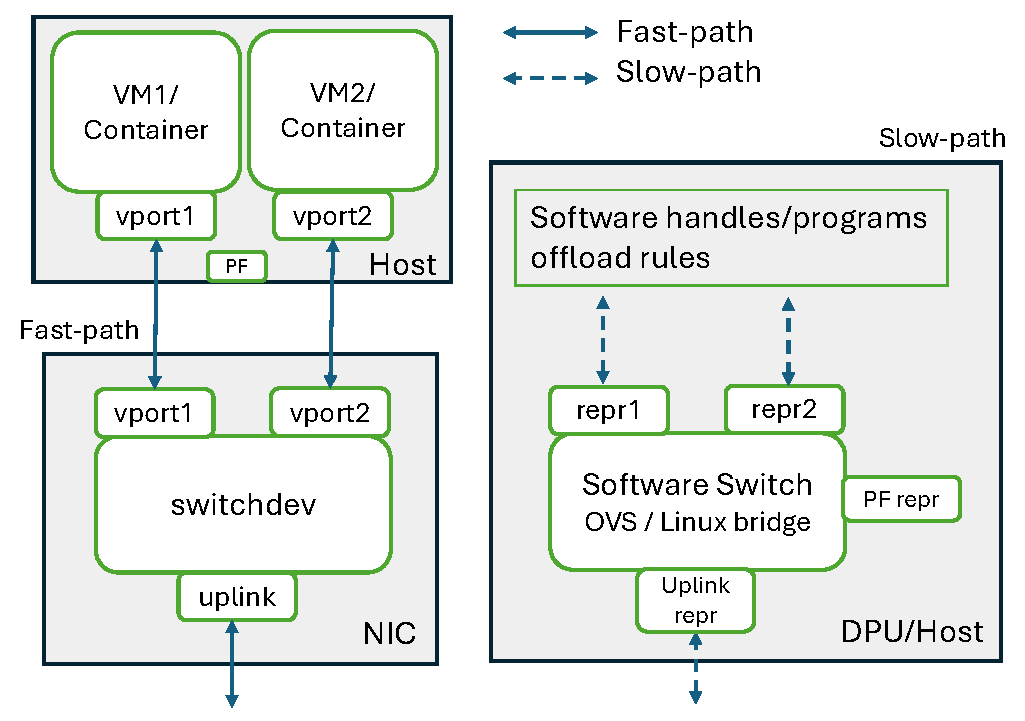
\includegraphics[width=3.4in]{arch.pdf}
\caption{The fast and slow path model. The switchdev in NIC is the fast path handling
hardware offloaded traffic among VFs/SFs, and the DPU which contains representor netdevs and software switch handles the slow path traffic.}
\label{fig:arch}
\end{figure}

%This post an important question: how much memory buffer does a representor
%netdev needs to pre-allocate for bursty traffic?
\iffalse
most of these representor netdevs' RX DMA memory
is idle when flows are forwarded directly in hardware to VFs.
In the recent case of smartnic or DPU (data processing unit) such as
Nvidia BlueField and Intel IPU, only the VFs and SFs and a light-weight PF
is exposed to the host side, the PF and representors are created in the
embedded CPU of the smartNIC.
The SmartNIC usually has less memory resources, Nvidia BlueField 3 has
32GB and Intel IPU has NGB, which makes the memory resource more precious.

In this talk we address the memory utilization challenges in DPU, by
first going through all existing solutions in different vendor drivers,
intel, nvidia, broadcom, netronme, and sfc. And we present the shared
memory pool design and implementation.
We should that by sharing the memory 
\fi

\section{Background}

\subsection{Eswitch and Switchdev Mode}
An eSwitch, or embedded switch, is a hardware component within modern network
controllers, such as the Intel® Ethernet Controller E810. It is also known as
a Virtual Ethernet Bridge (VEB). The eSwitch is managed by the Physical Function (PF)
driver of the Ethernet or in the case of SmartNIC, managed by the ECPF (Embedded CPU
s PF) that runs in the smartNIC's core. Eswitch can operate in two modes:
Legacy mode and Switchdev mode.

Legacy mode operates based on traditional MAC/VLAN steering rules. Switching
decisions are made based on MAC addresses, VLANs, etc. There is limited ability
to offload switching rules to hardware.
On the other hand, switchdev mode allows for more advanced offloading
capabilities of the E-Switch to hardware. In switchdev mode, more switching
rules and logic can be offloaded to the hardware switch ASIC, for example
push and pop tunneling protocol, connection tracking, etc.
This mode requires a slow path, software components such as OVS or
Linux bridge, and representor netdevices that handle miss traffic,
the flows that can not be offloaded or miss the hardware flow table
lookup, the slow path of VFs or SFs of the device.
% $$:`Documentation/networking/switchdev.rst <switchdev>` and
%:ref:`Documentation/networking/representors.rst <representors>`.
% devlink dev eswitch show
% devlink dev eswitch set mode switchdev
% need to disable OVS hwoffload
% so it's the iperf TX traffic on VF port that's going to overflow the PF's rxq

\subsection{Representors}
\begin{figure}[h]
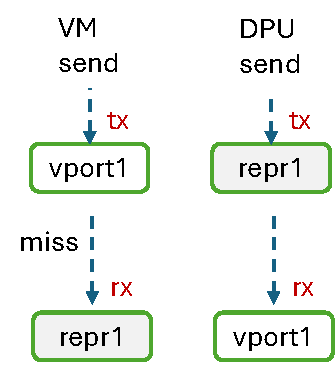
\includegraphics[width=3in]{pipe.pdf}
\caption{.}
\label{fig:arch}
\end{figure}

A vport can be PFs (used by administrator), or VFs or SFs (assigned to VMs
or containers). When the hardware offload table is empty, all packets are 
processed by the slow path. Representor netdev and vport are like a linux
pipe, shown in Figure~\ref{fig:pipe}: packets transmitted by the representor
netdev are delivered to its vport; packets transmitted by the vport are
received by the representor netdev, if it fails to match any offload rule.

% an end-to-end example
For example in Figure~\ref{fig:arch}, VM1 would like to setup a new TCP
connection to VM2. The first TCP syn packets sent from VM1 will miss the
NIC switchdev's flow table, due to no match, and arrives at the receive
queue of vport1's corresponding representor netdev, repr1.
OVS in this case, with hardware-offload enabled, will parse the protocol
and insert an offload rule, using Linux tc-flower interface.
In addition, OVS also forwards/sends the packet to the repr2 port, which
will deliver the packet to vport2's receive queue at VM2.
While VM2 receives the TCP syn from VM1, VM2 replies with SYN+ACK, and
again goes through the slow path. Until the connection is established
and flow rules are in NIC's flow table, the TCP data stream will be
going through the fast-path in NIC, and OVS in DPU no longer involves
in any packet processing.

Note that the behavior of the slow-path (representor ports and software
switch) should be the same as fast-path (vports and switchdev).
And because representor and vport are acting like pipe, so an OpenFlow
rule on a representor netdev applies to a packet on its
receive path is the same as it applies on vport's transmit path.

\iffalse
When the system boots, and before any offload is configured, all packets from
the virtual functions appear in the networking stack of the PF via the
representors.
The PF can configure standard Linux forwarding between representors, the uplink
or any other netdev (routing, bridging, TC classifiers).
Thus, a representor is both a control plane object (representing the function in
administrative commands) and a data plane object (one end of a virtual pipe).
\fi

\subsection{RX}
A network device driver consists of several channels and each channel/queue
represents an NAPI context and a set of queues that trigger that IRQ.
devlink-sd considers only the *regular* RX queue in each channel,
e.g., mlx5's non-regular RQs such as XSK RQ and drop RQ are not applicable
here. Each device driver receives packets by setting up RQ, and
each RQ receives packets by pre-allocating a dedicated set of rx
ring descriptors, with each descriptor pointing to a memory buffer.
The ``shared descriptor pool`` is a descriptor and buffer sharing
mechanism. It allows multiple RQs to use the rx ring descriptors
from the shared descriptor pool. In other words, the RQ no longer has
its own dedicated rx ring descriptors, which might be idle when there
is no traffic, but it consumes the descriptors from the descriptor
pool only when packets arrive.

The shared descriptor pool contains rx descriptors and its memory
buffers. When multiple representors' RQs share the same pool of rx
descriptors, they share the same set of memory buffers. As a result,
the heavy-traffic representors can use all descriptors from the pool,
while the idle, no-traffic representor consumes no memory. All the
descriptors in the descriptor pool can be used by all the RQs. This
makes the descriptor memory usage more efficient.


% explain eswitch, virtual port vport, representors, and port
% eswitch has vport
% vport nic 
As software-defined network and standards such as OpenFlow or tc-flower
requires more and more performance, network card vendors started to offer
complex virtualization capabilities than the legacy layer 2 mac/vlan switch
SR-IOV features, this leads to many new features and design in hardware offload
and device abstraction in Linux kernel.
This section talks about switchdev mode, the mode that enables
modern advanced hardware offloading capabilities as a hardware switch device,
and its data plance port function, vport or virtual port, and the vport's
control plane object, called representors.

\section{Design}
table here shows existing driver's implementation~\cite{buffersize}
\subsection{Nvidia mlx5 driver}
\subsection{Intel ice driver}
\subsection{Devlink Interface}

\section{Challenges}
\section{Thanks}

\subsection{Length of Papers}
A variety of paper lengths will be accepted under different categories. Please note that submission lengths must be all inclusive (including references, biographies and acknowledgements).
\begin{itemize}
\item Long paper submissions can be up to 8 pages in the ISEA2015 template format.
\item Art and Research short paper submissions can be up to 4 pages in the ISEA2015 template format.
\item Extended abstract submissions can be up to 2 pages in the ISEA2015 template format.
\item Round tables and square panel submissions can be up to 2 pages in the ISEA2015 template format.
\item Institutional presentation submissions can be up to 2 pages in the ISEA2015 template format.
\end{itemize}

\section{Style and Format}
Templates that implement these instructions can be retrieved electronically at {\small \tt http://isea2015.org}

\subsection{Layout}

Print manuscripts two columns to a page, in the manner in which these instructions are printed. The exact dimensions for pages are:
\begin{itemize}
\item left and right margins: 0.75''
\item column width: 3.31''
\item gap between columns: 0.38''
\item top margin—first page: 1.25''
\item top margin—other pages: 0.75''
\item bottom margin: 1.25''
\end{itemize}

\subsection{Format of Electronic Manuscript}

For the production of the electronic manuscript, you must use {\em Adobe's Portable Document Format} (PDF). Additionally, you must specify the American {\em letter} format (corresponding to 8-1/2'' x 11'') when formatting the paper.

\subsection{Blind Review}

All papers will be reviewed in a single blind manner.  You are at liberty to include your affiliation and cite your papers in a natural manner, and you are also at liberty to anonymize the text if you so desire, in which case, keeping your identity secret is your responsibility.

\subsection{Title and Author Information}

Center the title on the entire width of the page in a 16-point bold font. Below it, center the author name(s) in a 12-point bold font, and then center the address(es) in a 9-point regular font. Credit to a sponsoring agency can appear in the Acknowledgment Section described below.

\begin{figure}[h]
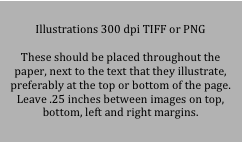
\includegraphics[width=3.31in]{figure.png}
\caption{This is an example of figure caption. Note that all figures, and tables are to be referenced in the text. \copyright Respect Copyright.}
\end{figure}

\subsection{Abstract}

The title ``Abstract'' should be 10 point, bold type, centered at the beginning of the left column. The body of the abstract summarizing the thesis and conclusion of the paper in no more than 200 words should be 9 point, justified, regular type.

\subsection{Text}

The main body of the text immediately follows the abstract. Use 10-point type in {\em Times New Roman} font.

Indent when starting a new paragraph, except after major headings. 

\subsection{Headings and Sections}

When necessary, headings should be used to separate major sections of your paper. (These instructions use many headings to demonstrate their appearance; your paper should have fewer headings.

\subsubsection{Section Headings}

Print section headings centered, in 12-point bold type in the style shown in these instructions. Your body text should be 10 point, justified, single space. Do not number sections.

\subsubsection{Subsection Headings}

Print subsection headings left justified, in 11-point bold type and mixed case (nouns, pronouns, and verbs are capitalized). They should be flush left. Your text should be 10 point, justified, single space. Do not number subsections.

\subsubsection{Subsubsection Headings}

Print subsubsection headings inline in 10-point bold type. Do not number subsubsections.

\subsubsection{Special Sections}

You may include an unnumbered acknowledgments section, including acknowledgments of help from colleagues, financial support, and permission to publish.

The references section is headed ``References,'' printed in the same style as a section heading. A sample list of references is given at the end of these instructions.  Note the various examples for books, proceedings, multiple authors, etc. 

\subsection{Footnotes}

If footnotes are necessary, place them at the bottom of the page in 9-point font. Refer to them with superscript numbers.\footnote{This is how your footnotes should appear.} Separate them from the text by a short horizontal line. 

\subsection{Itemized Lists}

Itemized lists shall use the en-dash as item. Let’s take the case of URL, automatic links and punctuation as an example:
Turn off the automatic linking feature for URLs in Word.

Quotations: For direct quotations remember to use ``double inverted commas.'' Quotations must be carefully transcribed and accurate. 

Periods and commas go inside quotation marks. This applies to ``double inverted commas,'' as well as single `inverted commas,' and to the use of a full stop as in the ``following example.'' 

Parenthesis: When an entire sentence is enclosed in parentheses, the punctuation mark belongs inside the closing parenthesis as in this example: applying this may be difficult at times. (We think it is important.)

\begin{itemize}
\item The punctuation mark belongs outside the closing parenthesis if the brackets are within the sentence as in this example: applying this may be difficult at times, but good results are guaranteed (and this is important).
\item Use en dashes with spaces -- like this -- to set off phrases. En dashes are moreover placed between digits to indicate a range (1--10 October; pp. 25--30). You can type an en dash with ALT + 0150 (in the numeric keypad) in Windows, or OPTION + HYPHEN in Mac.
\end{itemize}

\subsection{Quotations and Extracts}
Indent long quotations and extracts by 10 points at left margins.

\section{Acknowledgments}
The preparation of these instructions and the \LaTeX{} and Word files was facilitated by borrowing from similar documents used for ICCC proceedings.

\begin{figure*}

\includegraphics[width=\textwidth]{two-column-figure.png}
\caption{Example of a double-column figure with caption. \copyright Respect Copyright.}
\end{figure*}

\section{Bibliography}
The title ``Bibliography'' should be 12 point, bold style, centered. Using 9 point, regular type, list your bibliography in alphabetical order by family name, after the references. The difference between a reference list and a bibliography is that in your references, you list all the sources you directly referred to in the body of your writing in numerical order, whereas a bibliography includes an alphabetical listing of all those authors and sources that you have consulted while writing your essay. Use the same format as for the references otherwise. Those using Latex will follow the usual cite command format \cite{boden92}.

\section{Author(s) Biography(ies)}
The title ``Author(s) Biography(ies)'' should be 12 point, bold style, centered. Using 9 point, regular type, biographies should be no longer than 150-word count.

\section{Questions?}

For technical questions about Microsoft Word formatting please seek online tutorials. For other questions about your manuscript please contact: {\tt ISEA2015-info@sfu.ca}


\bibliographystyle{isea}
\bibliography{isea}


\end{document}
%challenges and takeaways
%\begin{figure}[h]
%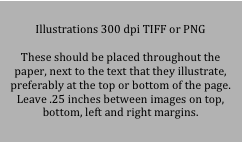
\includegraphics[width=3.31in]{figure.png}
%\caption{This is an example of figure caption. Note that all figures, and tables are to be referenced in the text. \copyright Respect Copyright.}
%\end{figure}
